\documentclass{beamer}
%\setbeameroption{show notes on second screen=right} % Both
\setbeameroption{hide notes} % Only slides
%\setbeameroption{show only notes} % Only notes
% Theme choice:
\usetheme{Antibes}
\usepackage{tikz-feynman}
\usepackage{array}
\usepackage{animate}
\usepackage{amsmath}
\usepackage{cancel}
\usepackage{multicol}
\usepackage{physics}
\usepackage{graphicx}
\usepackage{amssymb}
\usepackage{hyperref}
%\hypersetup{colorlinks = true,linkcolor = black,filecolor= black,urlcolor= black}
\usepackage{cancel}
\usepackage{subcaption}
\usepackage{comment}
\usepackage[backend=bibtex,bibencoding=utf8,style=authortitle,citestyle=authortitle]{biblatex}
\addbibresource{library}
\AtEveryBibitem{%
	\clearname{translator}%
	\clearlist{publisher}%
	\clearfield{pagetotal}%
}
\usepackage{xparse}
\usepackage{svg}
\usepackage[toc,page]{appendix}
\author{Vo Chau Duc Phuong}
% Title page details: 
\title{Calculation of the Linear-Absorption Spectrum of\\ an Ideal Two-Dimensional System of $\mathrm{MoS}_2$}
\author{Vo Chau Duc Phuong \inst{1} \\
	{\and} \\
	{\textit{Supervisors}} \\
Dr. Huynh Thanh Duc \inst{2}}
\institute[shortinst]{\inst{1} University of Science, Ho Chi Minh city\and %
\inst{2} Institute of Applied Mechanics and Informatics}
\date{14/07/2024}
\logo{\large \LaTeX{}}

\begin{document}
	\small
	% Title page frame
	\begin{frame}
		\titlepage
		\note{Good day, teachers and fellow students. Now is my turn to present my work, on the "Calculation of the linear absorption spectrum of MoS2".}
	\end{frame}
	
	% Remove logo from the next slides
	\logo{}
	
	
	% Outline frame
	\section*{Outline}
	\begin{frame}{Outline}
		\tableofcontents
		\note{First, let's go through the overview of this presentation. I will go through:}
		\note[item]{the overview of the compound, its properties, and why we choose this path.}
		\note[item]{Then, introducing the model we are using, the equations and the outcome we need to calculate.}
		\note[item]{after that, talk and discussion about the results}
		\note[item]{finally, I will summary and talk about further research}
	\end{frame}
	
	\section{Overview}
	% Lists frame
	\begin{frame}{Transition Metal Dichalcogenides Monolayers}
		Group VI-B Transition Metal Dichalcogenides (TMD) are compound semiconductors of the type $MX_2$. :
		\begin{figure}
			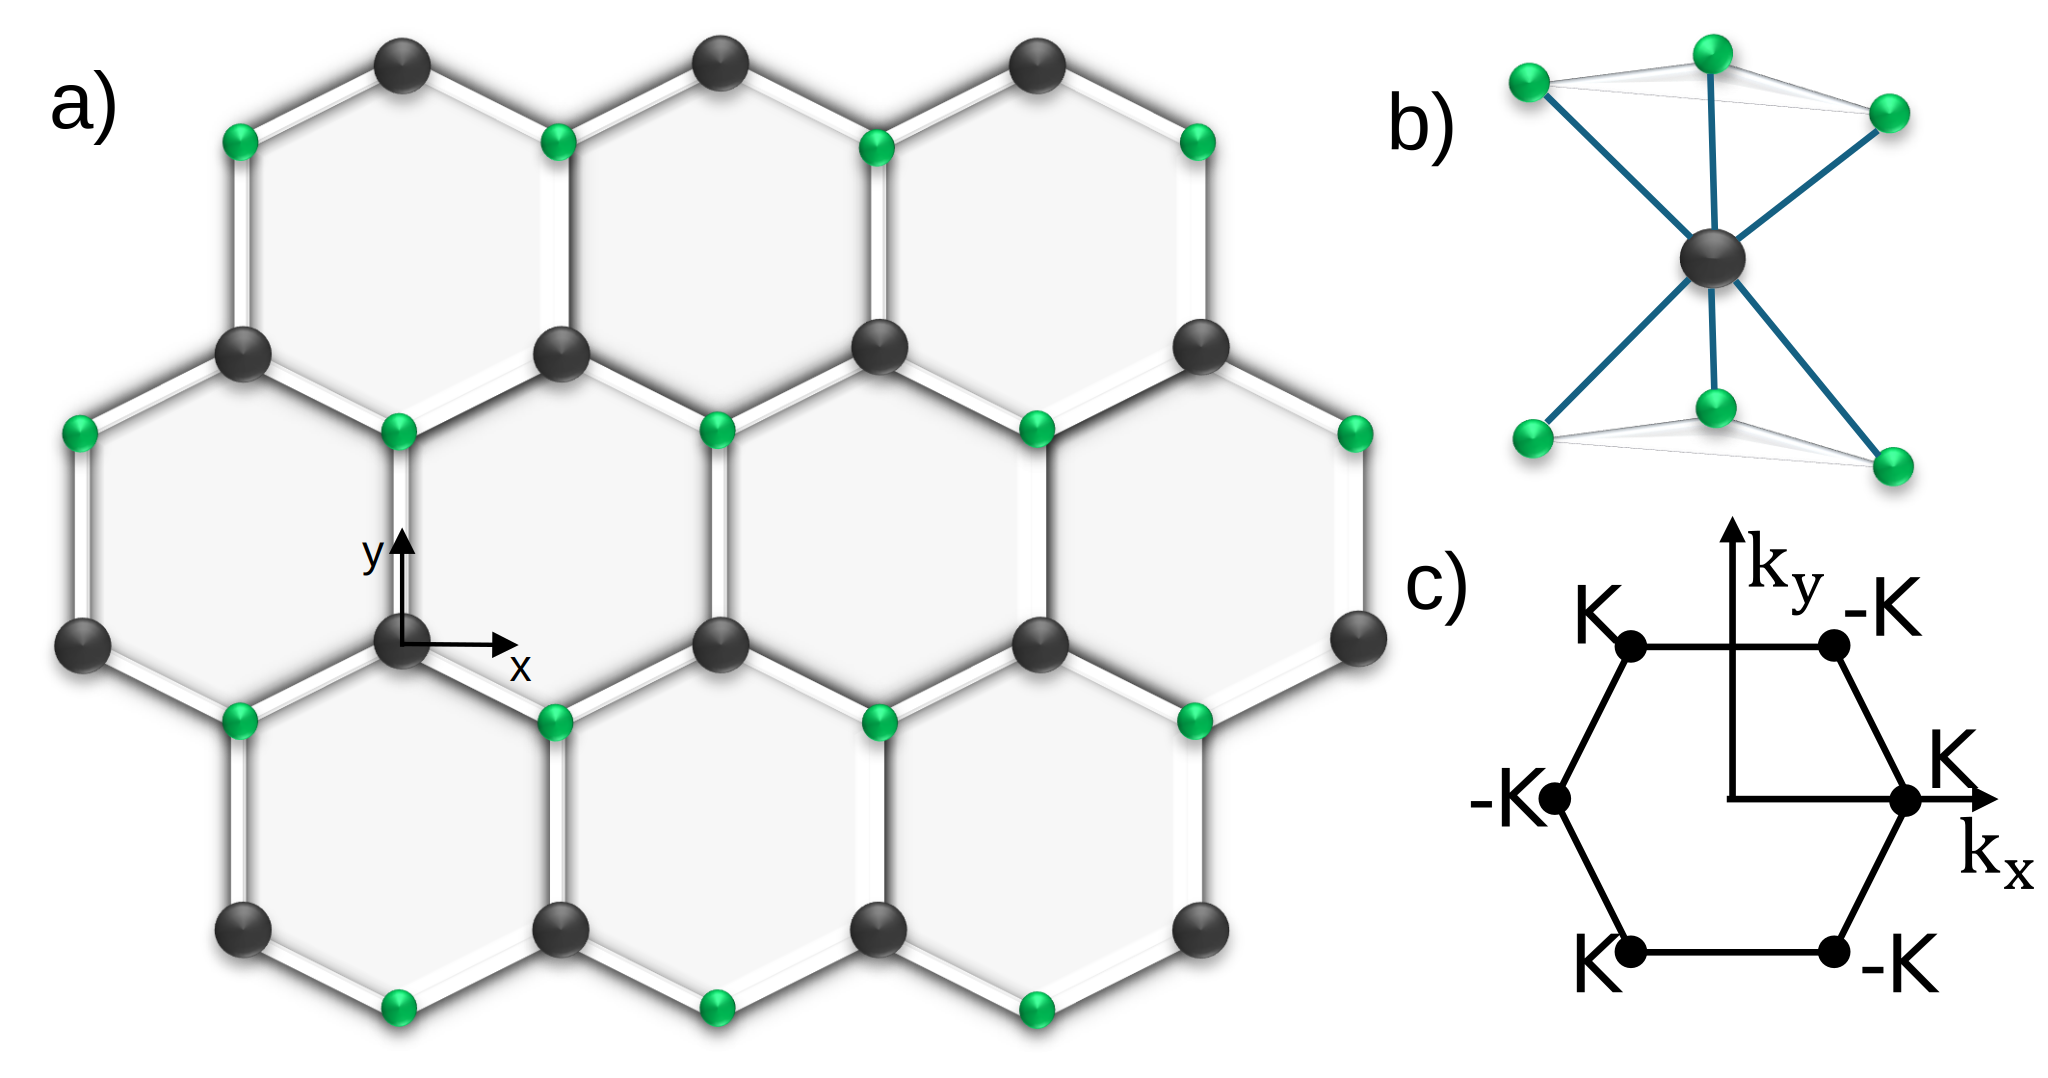
\includegraphics[width=0.5\linewidth]{images/RS.pdf}
			\caption{Structure of TMD and its first Brillouin Zone. $M$ is Transition Metal atom (black dots), $X$ is Dichalcogenide atom (green dots)}
		\end{figure}
		\note[item]{Transition metal dichalcogenides, which I will refer to as TMD, are compounds of the type MX2.}
		\note[item]{TMD has a layered structure, so it's easy to create a monolayer by extracting the layers like a Lego structure. The monolayer structure is like a sandwich, with chalcogenide layers above and below and the transition metal layer in between, you can see in figure a from top and b from side in here.}
		\note[item]{The first Brillouin zone, which I will abbreviate as BZ, has a hexagonal shape, show in figure c.}
	\end{frame}

	\begin{frame}{Transition Metal Dichalcogenide Monolayers}
\begin{block}{Properties}
\begin{itemize}
\item They are stable in both mono- and few-layer in the air at room temperature. \\
\item They are semiconductors with a direct band gap in visible light range.
\item Their crystal structure has no center of inversion.\\
\item Strong spin-orbit coupling (SOC) in TMD monolayers leads to spin splitting of hundreds meV.
\end{itemize}
\end{block}
$\Rightarrow$ Promising materials in electronic and optoelectronic applications (for example: solar cells with energy conversion efficiency surpassing the Schockley-Queisser limit).
\note{The monolayer of TMD has some interesting properties, such as:}
\note[item]{Stable in the air at the room's temperature}
\note[item]{direct band-gap in the visible light range}
\note[item]{"no center of inversion"}
\note[item]{strong spin-orbit coupling. These properties of TMD promise it will become a gift material in electronic and optoelectronic.For example: making solar cells with aiming to surpass the Schockley-Queisser limit.}
	\end{frame}
	\begin{frame}{Exciton Binding Energy In TMD}
Exciton binding energy can be extracted from the linear absorption spectrum
\begin{block}{Overview}
\begin{itemize}
\item TMD is a low-dimensional material $\to$ huge exciton binding energy in compared with bulk semiconductors $\to$ electron-hole Coulomb interaction need to be calculated and taken into account.
\item Early theories predict large binding energy ($0.5-1$ eV) in compare with experiment ($0.2-0.5$ eV) $\Rightarrow$ more precise calculations to match with the experiments.
\item Theories only fit bandstructure around highly symmetry points such as $K/K'$, not on entire BZ $\Rightarrow$ a models for fitting in the entire BZ.
		\end{itemize}
\end{block}
\note[item]{In this work, we calculate the linear absorption spectrum to obtain the exciton binding energy. Since TMD is a low-dimensional material, it results in a huge exciton binding energy (about two magnitude orders compared with other bulk semiconductors).}
\note[item]{Early theories predict binding energy is too large compared with the experiment, so we need to calculate it to match with the experiment.}
\note[item]{In this work, we choose a tight-binding model, which is developed to fit in the entire BZ.}
	\end{frame}
	% Blocks frame
	\section{Method}
	\subsection{Three-band Tight-binding Model}
	\begin{frame}
		Tight-binding (TB) wave function has the form:
		\begin{equation}
			\ket{\psi_{\lambda \textbf{k}}(\textbf{r})} = \sum_{\alpha} c_{\lambda \alpha} (\textbf{k}) \sum_{\textbf{R}} e^{i\textbf{k}\textbf{R}} \ket{\phi_{\alpha}(\textbf{r}-\textbf{R})}.
		\end{equation}
		The Time-independence Schrödinger equation:
		\begin{equation*}
			H_{1e} \sum_{\alpha} c_{\lambda \alpha} (\textbf{k}) \sum_{\textbf{R}} e^{i\textbf{k}\textbf{R}} \ket{\phi_{\alpha}(\textbf{r}-\textbf{R})} = \varepsilon_{\lambda} (\textbf{k}) \sum_{\alpha} c_{\lambda \alpha} (\textbf{k}) \sum_{\textbf{R}} e^{i\textbf{k}\textbf{R}} \ket{\phi_{\alpha}(\textbf{r}-\textbf{R})}.
		\end{equation*}
		Multiply with $\bra{\phi_{\beta}}$ on the left and take integral over $\textbf{r}$
		\begin{equation}
			\sum_{\alpha} [H^{TB}_{\beta \alpha}(\textbf{k}) - \varepsilon_{\lambda}(\textbf{k})\delta_{\beta\alpha}]c_{\lambda \alpha}(\textbf{k}) = 0.
		\end{equation}
		Tight-binding Hamiltonian matrix elements:
		\begin{equation}
			H^{TB}_{\beta \alpha}(\textbf{k}) = \sum_{\textbf{R}} \bra{\phi_{\beta} (\textbf{r})} H_{1e}\ket{\phi_{\alpha}(\textbf{r}-\textbf{R})}.
		\end{equation}
\note{The tight-binding wave function has the form of Eq. (1). Including it into the time-independence Schrödinger to get Eq. (2) and Eq. (3).}
	\end{frame}
	\begin{frame}
Use basic functions of d-type orbitals: $$\ket{\phi_1} = d_{z^2}, \ket{\phi_2} = d_{xy}, \ket{\phi_3} = d_{x^2- y^2}.$$\\Three-band TB Hamiltonian with SOC has the form:
		\begin{equation*}
			H^{TB}_{6\times 6}(\textbf{k}) = \begin{bmatrix}
				H^{TB}_{3\times 3}(\textbf{k}) + \gamma L_z & 0\\ 0& H^{TB}_{3\times 3}(\textbf{k}) - \gamma L_z
			\end{bmatrix}, \quad L_z= \begin{bmatrix}
			0 & 0 & 0\\
			0 & 0 & i\\
			0 & -i& 0
			\end{bmatrix}.
		\end{equation*}
\note{The model we use in this work is called the three-band tight-binding models, It using basic function of 3 d-type orbitals as shown. The full Hamiltonian at a k-point is a 6 by 6 matrix when take spin orbit coupling into account.}
	\end{frame}
	\begin{frame}
		\begin{figure}
			\caption{Band structure of $MoS_2$ monolayer
\footcite{liu_three-band_2013}}
			\includegraphics[width=0.75\linewidth]{images/BS.pdf}
		\end{figure}
	\note{The BS of this model is shown here, which huge band split (about 144 meV) at K and K' points. In this work, we will focus on the transition between the valence bands and the first pair of conduction bands.}
	\end{frame}
	\subsection{Semiconductor Bloch Equations}
	\begin{frame}
	\begin{block}{Multiband semiconductor Bloch equations (SBE) with Coulomb interaction in Hatree Fock approximation:}
	\begin{align}
		\dv{ }{t}\rho_{\lambda \lambda'} (\textbf{k},t) = &-\frac{i}{\hbar} (\varepsilon_{\lambda}(\textbf{k}) -\varepsilon_{\lambda'}(\textbf{k}))\rho_{\lambda \lambda'} (\textbf{k})\nonumber\\
		& -i \sum_{\mu} (\Omega_{\lambda \mu}(\textbf{k})\rho_{\mu \lambda'}(\textbf{k},t) -\rho_{\lambda \mu}(\textbf{k},t)\Omega_{\mu \lambda'}(\textbf{k}))\\
		& + \frac{\rho_{\lambda \lambda'}(\textbf{k},t)}{T_2}(1-\delta_{\lambda\lambda'}),\nonumber
	\end{align}
	\end{block}
	where
	\begin{small}
	\begin{align}
		\Omega_{\mu \nu}(\textbf{k}) &= \frac{1}{\hbar} \bigg(\frac{e}{m}\textbf{A}(t)\textbf{p}_{\mu \nu}(\textbf{k}) - \sum_{\alpha \beta \textbf{q}} W^{\alpha \mu \beta\nu}_{\textbf{k},\textbf{k}+\textbf{q},\textbf{q}}\rho_{\beta\alpha}(\textbf{k}+\textbf{q})\bigg),\\
		\textbf{p}_{\mu\nu}(\textbf{k}) &= \frac{m}{\hbar}\sum_{\alpha,\beta} c^*_{\mu\alpha}(\textbf{k})\nabla_{\textbf{k}}H^{TB}_{\alpha\beta}(\textbf{k})c_{\nu\beta}(\textbf{k}),\\
		W^{\alpha \beta \gamma \delta}_{\textbf{k}, \textbf{k}',\textbf{q}} &= \frac{e^2}{2\varepsilon\varepsilon_0 L^2} \frac{1}{|\textbf{q}|}
\sum_{\mu,\nu} c^*_{\alpha\mu}(\textbf{k}+\textbf{q})c_{\delta\mu}(\textbf{k}) c^*_{\beta \nu}(\textbf{k}'-\textbf{q}) c_{\gamma \nu}(\textbf{k}')
	\end{align}
	\end{small}
	\note{Using the semiconductor Bloch equation (SBE), we solve it in the form of Eq. (4) to obtain the time-dependent evolution of density matrix elements.}
	\end{frame}
\subsection{Inter-band Polarization}
\begin{frame}
		\begin{multicols}{2}
Dipole matrix elements can be obtained through:
\begin{align}
&\vec{\xi}_{\mu\nu}(\textbf{k}) = \frac{-i\hbar}{m}\frac{\textbf{p}_{\mu\nu}(\textbf{k})}{\varepsilon_{\mu}(\textbf{k}) - \varepsilon_{\nu}(\textbf{k})}.\\
&\text{for } \mu \neq \nu \nonumber
\end{align}
Time-dependent interband polarization density:
\begin{align}
\textbf{P}(t) = &\frac{e}{L^2} \sum_{\textbf{k}} \Tr\bigg[\vec{\xi}(\textbf{k})\rho(\textbf{k},t)\bigg]\nonumber\\
= &\frac{e}{L^2} \sum_{\textbf{k}\lambda\lambda'}\vec{\xi}_{\lambda\lambda'}(\textbf{k})\rho_{\lambda'\lambda}(\textbf{k},t).
\end{align}
\columnbreak
\begin{figure}
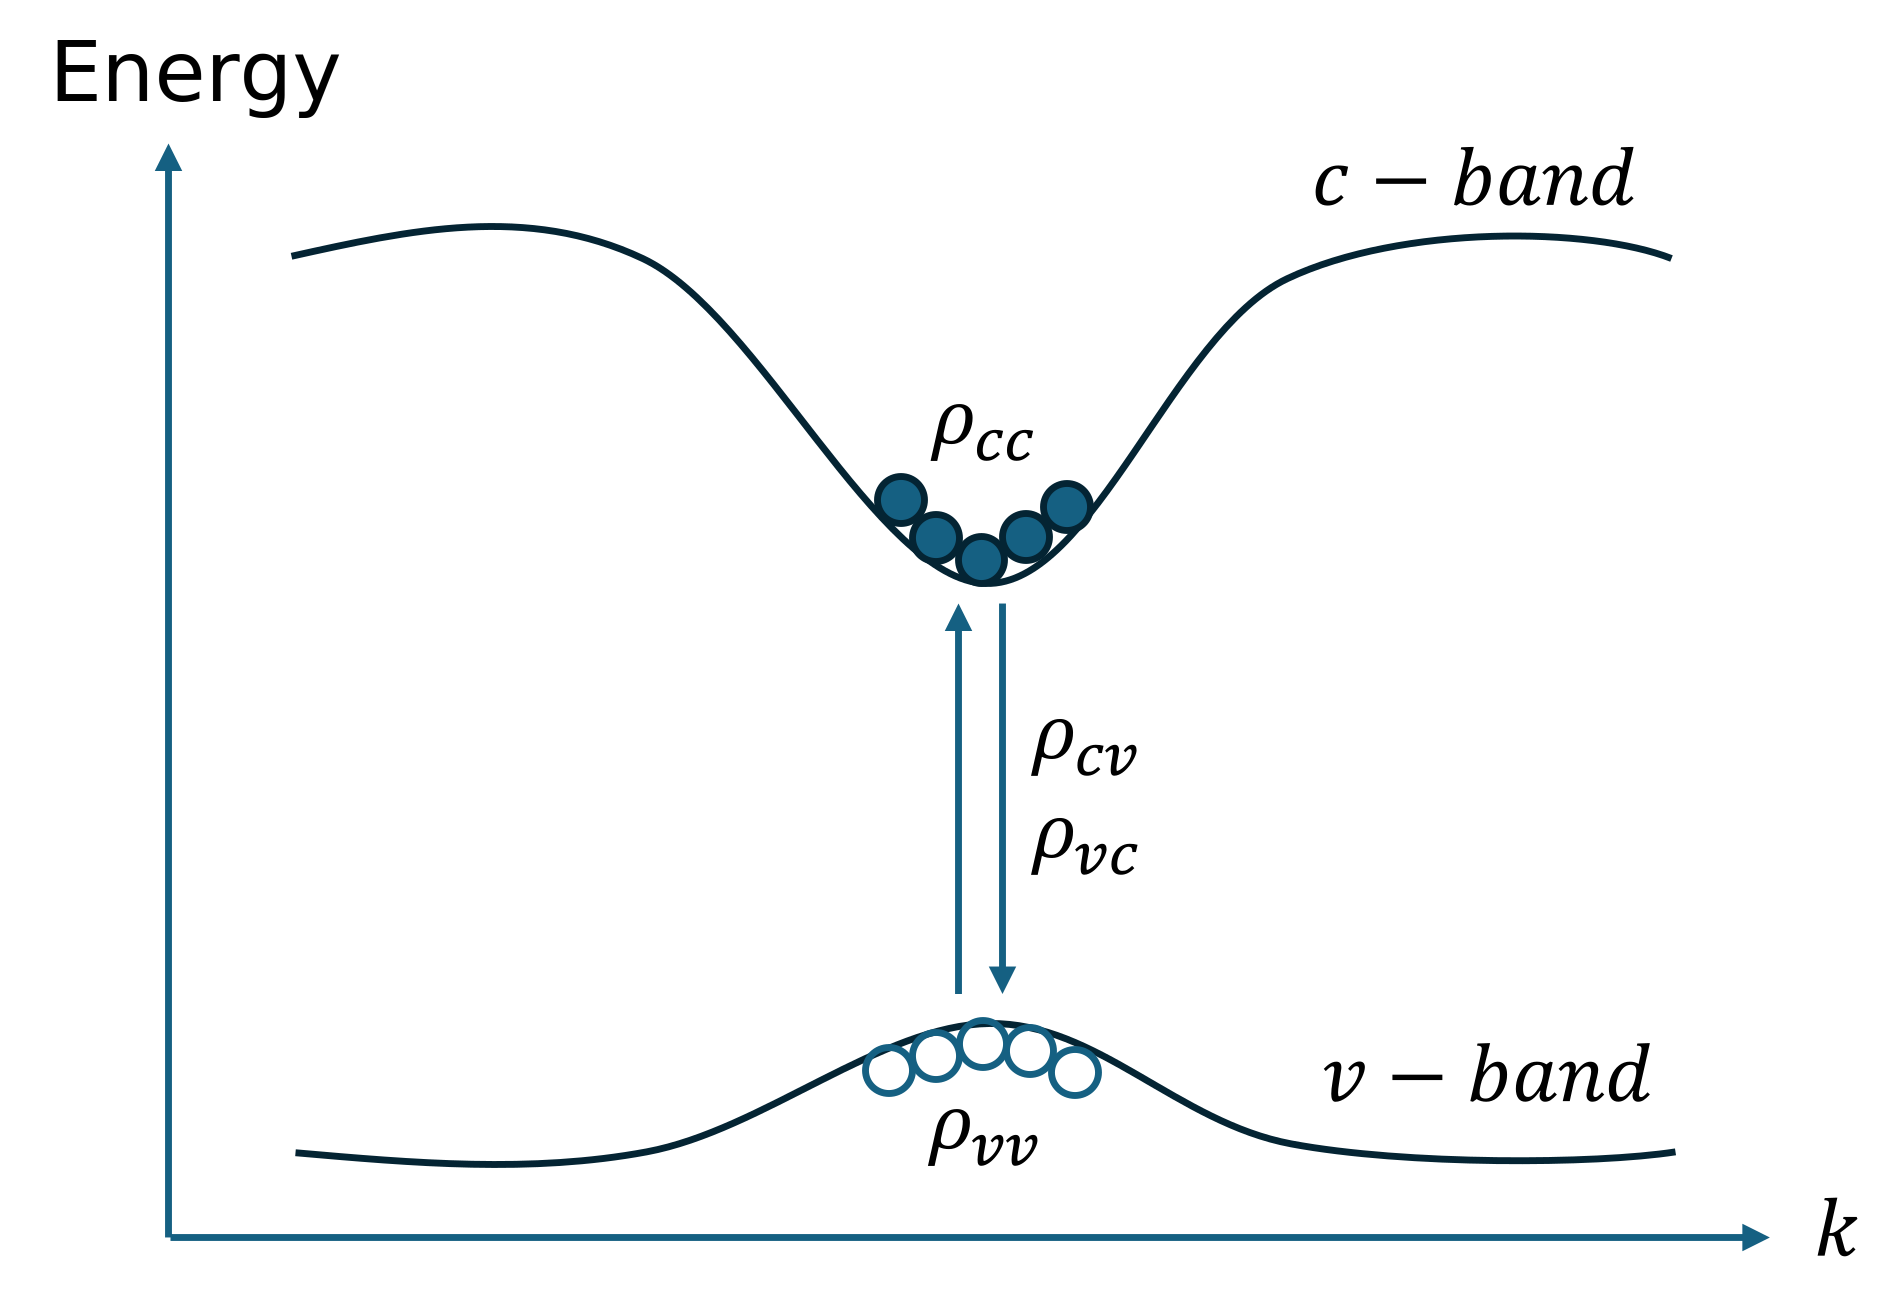
\includegraphics[width=1\linewidth]{images/cvbeamer.pdf}
\caption{Density matrix element illustration}
\end{figure}
	\end{multicols}
\note{Using the density and dipole matrix elements, we can obtain the time dependence interband polarization through Eq.(9)}
	\end{frame}
\section{Numerical Results}
	\begin{frame}{Numerical Evaluation of The Sum Over k-space}
		\begin{figure}
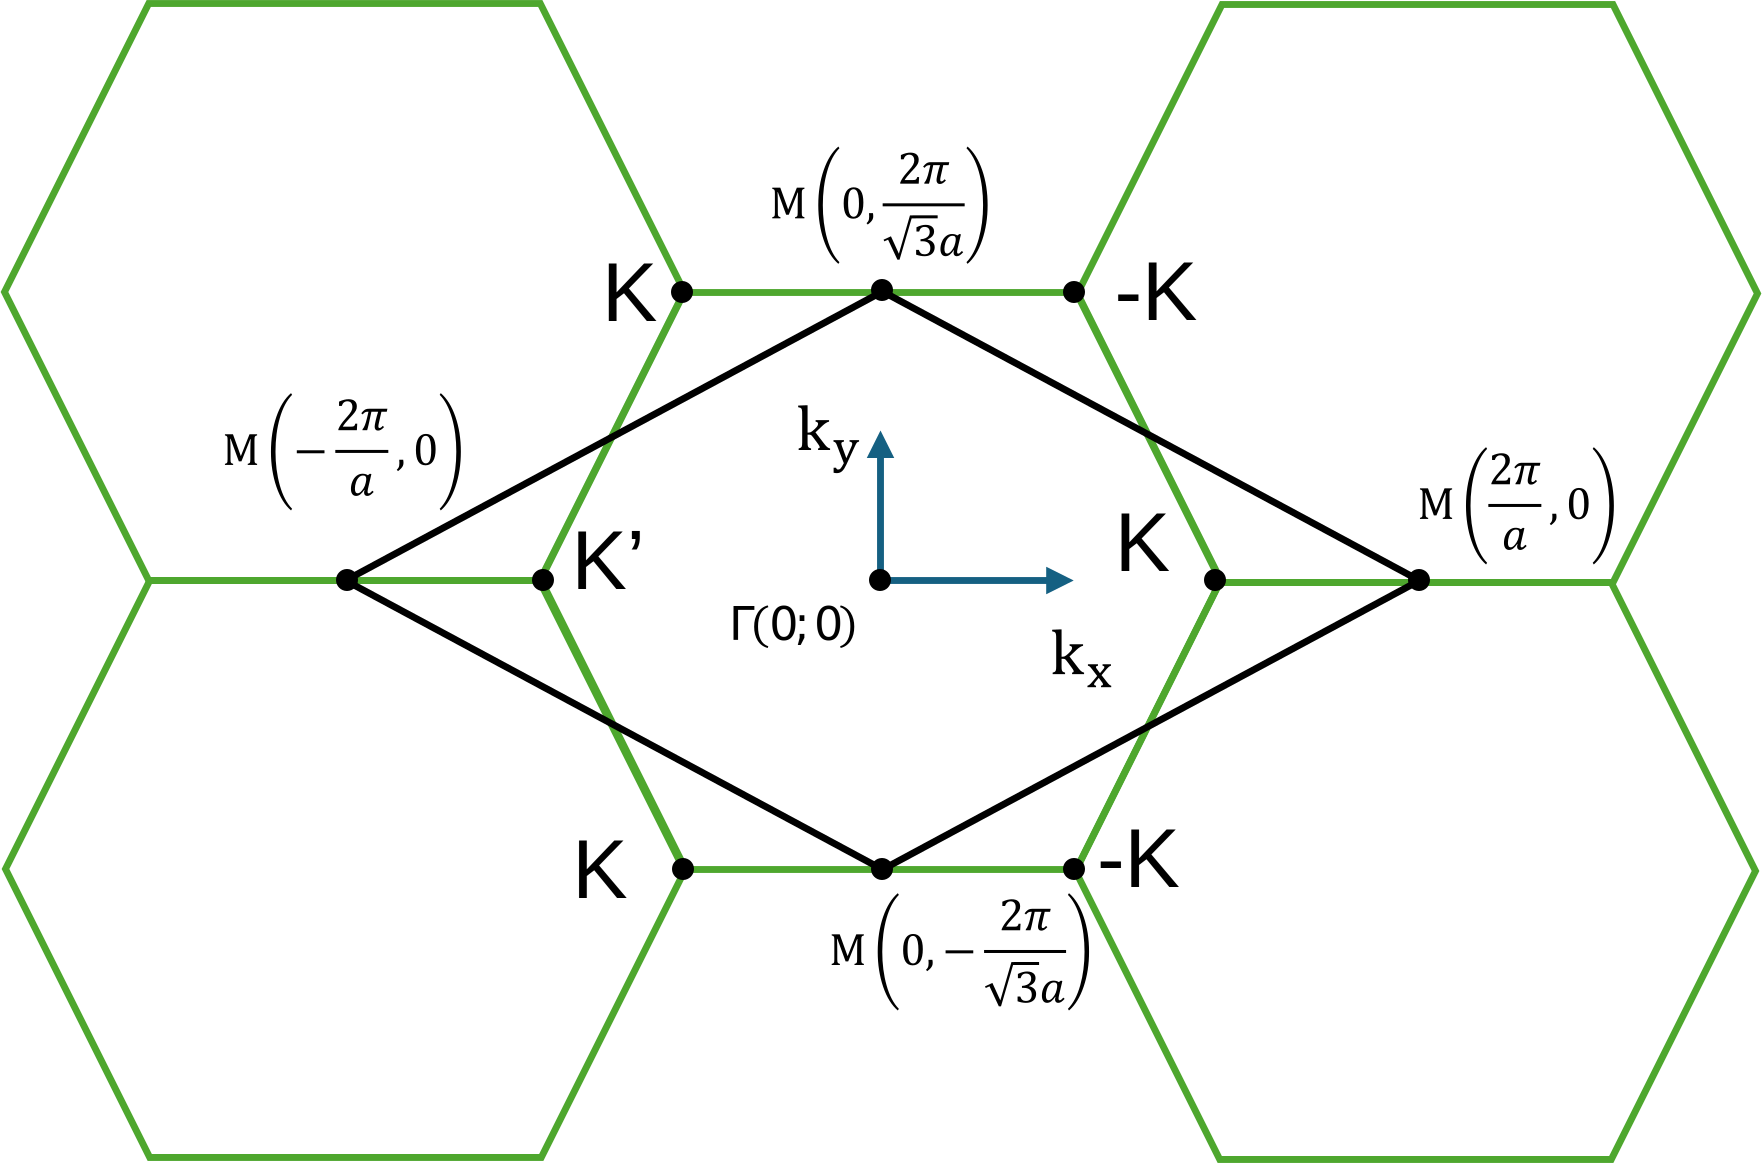
\includegraphics[width=0.5\linewidth]{images/Rhombus.pdf}
\caption{Rhombus primitive cell}
\end{figure}
		\begin{equation}
			\sum_{\textbf{k}} ... \to \frac{L^2}{4\pi^2} \int \int_{BZ} dk_x dk_y...
		\end{equation}
\note[item]{As I have mentioned above, The first Brillouin Zone of monolayer TMD have the shape of Hexagon. However, the hexagon is inconvenient for us when sampling the k-grid, so we will use the rhombus primitive cell with the same area as the hexagon.}
\note[item]{In order to evaluate the numerical results in the entire BZ, we approximate the sum by this integral.}
	\end{frame}
	\begin{frame}{k-Cutoff}
	\begin{figure}
		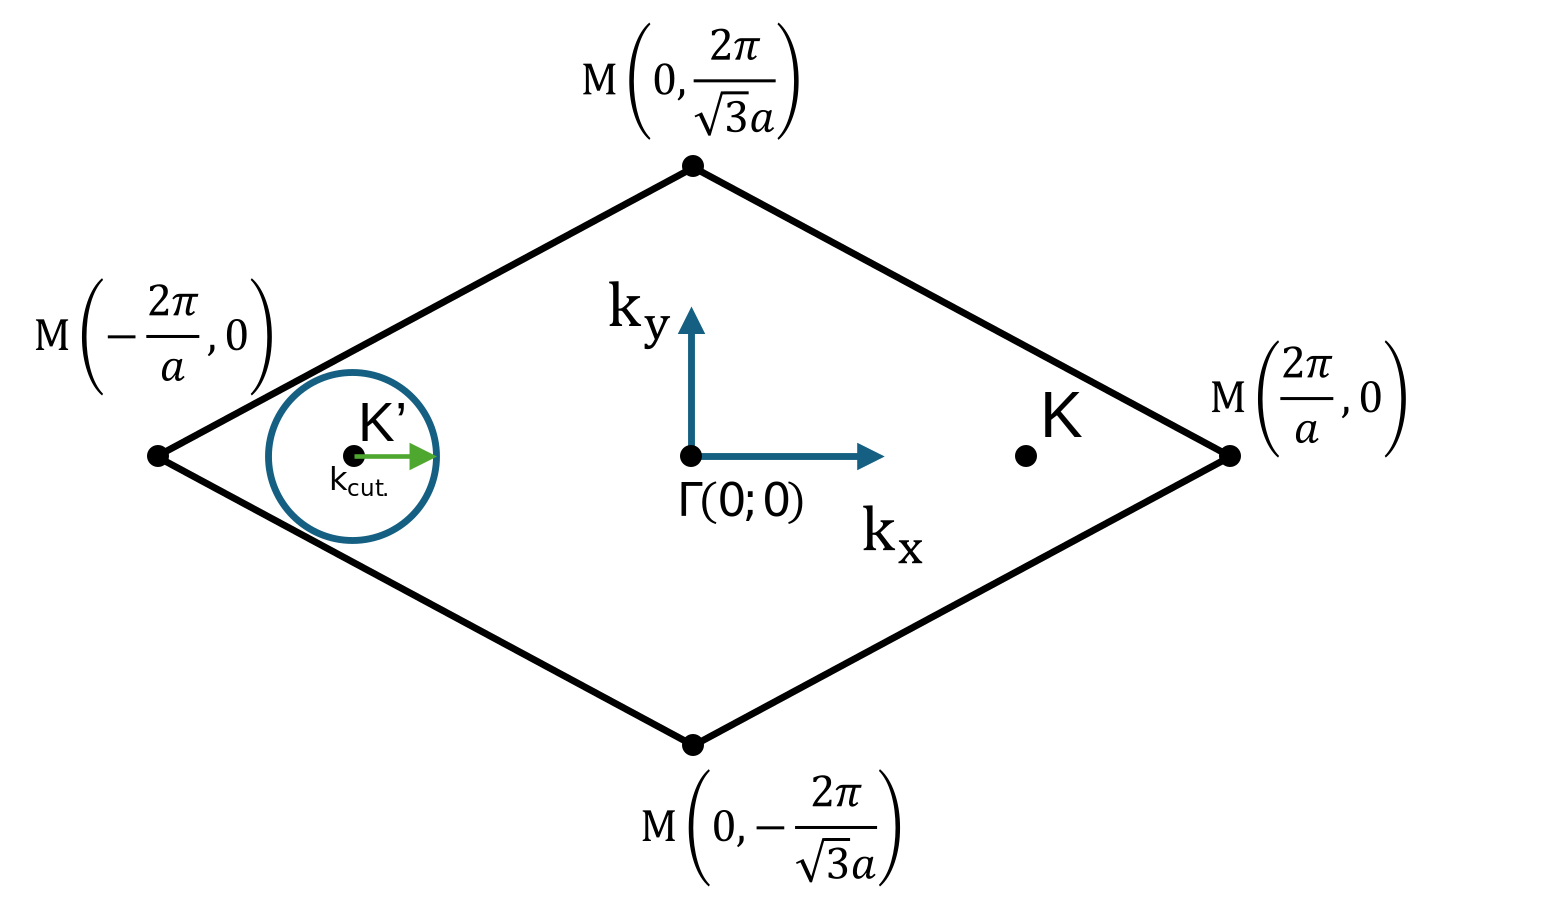
\includegraphics[width=0.75\linewidth]{images/kcutoff.pdf}
	\end{figure}
For k-points around \textbf{K}' point
	\begin{equation}
		W^{\alpha \mu \beta \nu}_{\textbf{k},\textbf{k}',\textbf{q}} \approx W^{\alpha \mu \beta \nu}_{\textbf{k},\textbf{k}',\textbf{q}} \theta(k_{cut.} - |\textbf{k} - \textbf{k}_{K'}|) \theta(k_{cut.} - |\textbf{k}' - \textbf{k}_{K'}|).
	\end{equation}
	The same for k-points around \textbf{K} point
	\note[item]{When considering the Coulomb interaction, it's essential to account for every k-point in the Rhombus primitive cell. However, including every k-point may result in an overwhelming workload for achieving convergence. For this reason, we employ a technique that focuses specifically on k-points around K and K'.}
	\note[item]{For instance, with the K' point, we draw a circle and calculate the Coulomb interaction only if both points fall within this circle. The same process applies to the K point.}
	\end{frame}
	\begin{frame}{Electromagnetic Field}
	\begin{multicols}{2}
The electric field has a Gaussian envelope form:
\begin{equation}
	\textbf{E}(t) = \textbf{E}_0 \cos(\omega_0 t)e^{-\frac{t^2}{\tau_L^2}}
\end{equation}
\begin{itemize}
	\item small $E_0: \rho_{cc}(\textbf{k}) \to 0$
	\item $\hbar \omega_0 = E_{gap.}$
	\item small $\tau_L \to $ rounder Fourier transform's peak around $\omega_0$
\end{itemize}
\columnbreak
\includegraphics[width=1\linewidth]{images/Eat.pdf}
Absorption coefficient\footcite{haug_quantum_2009}:
\begin{equation}
	\alpha(\omega) \propto \frac{P(\omega)}{E(\omega)}.
\end{equation}
	\end{multicols}
\note[item]{The polarized external field has a Gaussian envelope form with these properties to obtain the weak excitation limit for the linear absorption calculation.}
\note[item]{The absorption coefficient will be obtained by Eq. (13)}
\note[item]{P and E is Fourier transformation of polarization density and external field, respectively}
	\end{frame}
	\begin{frame}
		Experiment measure:
		\begin{multicols}{2}
		\begin{figure}
	\includegraphics[width = 1\linewidth]{images/Experiment.pdf}
	\caption{Measured Absorption Spectrum of $\mathrm{MoS}_2$ at $T=5K$  extracted from Ref.  \footcite{zhang_absorption_2014}} $E_{gap} = 2.15 \pm 0.06$ \(eV\)
	\end{figure}
Binding energy: \\
	$E_{bind.} = E_{gap} - E_{A} = 0.22$ \(eV\)
 \columnbreak
	\begin{itemize}
		\item Two resonance labeled by A ($1.93$ \(eV\)) and B ($2.1$ \(eV\)) are exciton peaks (band split due to SOC)
		\item Weak trion peak near A labeled by A' ($18$ \(meV\))
	\end{itemize}
To fit with experiment, we can change:
\begin{itemize}
\item Relative permittivity $\varepsilon$
\item Dephasing time $T_2$
\end{itemize}
	\end{multicols}
\note[item]{The experiment measurement gives us two peaks, labeled as A ($1.93$ \(eV\)) and B ($2.1$ \(eV\)), the binding energy will be obtain by extract the exciton peak from the bandgap energy}
\note[item]{they also have a weak trion peak in here.}
\note[item]{To fit with the measurement, we will investigate the relationship between relative permittivity and dephasing time T2 with linear absorption spectrum.}
	\end{frame}
\begin{frame}
\begin{figure}
	\includegraphics[width=0.8\linewidth]{images/varyT2.pdf}
\end{figure}
		
\begin{itemize}
\item Choosing the $T_2$ for clearer Exciton peak.
\item The bigger $T_2$, the clearer main Exciton peaks $\to $ confirm two peak.
\item At $T_2 = 30$ \(fs\) show other smaller peaks $\to $ predict other peaks.
\note[item]{As we vary T2, two peaks become clearer at bigger T2, which agrees with the measurement.}
\note[item]{We can also see smaller peaks, which are other exciton peaks but too small to appear in the measurement.}
\end{itemize}
\end{frame}
\begin{frame}
	\begin{center}		
		\includegraphics[width=0.8\linewidth]{images/varyepsilon.pdf}
	\end{center}
	\begin{itemize}
		\item Choosing the $\varepsilon$ for fitting with the experiment.
		\item For 3-band TB model: $\varepsilon \in (1.5,2.5)$ is in good agreement with exciton binding energy of $E_{bind.}= 0.2-0.5 eV$ 
	\end{itemize}
	\note[item]{The binding energy is affected through the relative permittivity, as we increase the epsilon, two peaks move to the right of the spectrum.}
	\note[item]{With the same epsilon equal to 2.5, we obtain the same results as the experiment, approximately 0.24 eV for the exciton binding energy.}
\end{frame}
	%\begin{frame}
	%\includegraphics[width=1\linewidth]{images/varynk.pdf}
	%\end{frame}
	\section{Summary and Outlook}
	\begin{frame}
	\begin{block}{Summary:}
\begin{itemize}
\item From three-band TB + SBE $\to $ Linear Absorption Spectrum
\item We confirm the Exciton binding energy in this model is in agreement with experimental data, and predict smaller exciton peaks.
\end{itemize}
	\end{block}
	\begin{exampleblock}{Further research:}
	\begin{itemize}
		\item High Harmonic Generation
		\item High-order Side-band Generation
		\item Photovoltaic effect
	\end{itemize}
\end{exampleblock}
	\begin{center}
		Thank you for your listening.
	\end{center}
	\note[item]{So far, we have used the three-band tight-binding model and semiconductor Bloch equations to calculate the linear absorption spectrum. We confirm that this model matches the results with the experiment data and also predicts smaller exciton peaks.}
	\note[item]{For further results, we can include the many-body interaction in calculating other phenomena for a realistic picture of TMD's properties.}
	\end{frame}
\end{document}